%% ============================================================
%%  CHAPTER 2 — Bounded Inquiry: Cell-Truth, Layered Receivers,
%%              and Mode–Methodology Equivalence
%% ============================================================

%% Local notation for this chapter.
%% \receiver, \Sfloor, \catpow, \OscRep, \CatRep, \PartRep inherited from Ch.1.
\providecommand{\Cell}{\mathcal{C}}
\providecommand{\Meth}{\mathfrak{M}}
\providecommand{\OutcomeX}{\mathcal{X}}
\providecommand{\NoiseFloor}{\beta}
\providecommand{\Know}{\mathrm{Know}}
\providecommand{\diam}{\mathrm{diam}}
\providecommand{\dom}{\mathrm{dom}}

\chapter{Bounded Inquiry: Cell-Truth, Layered Receivers, and Mode--Methodology Equivalence}
\label{ch:epistemology}

\papernote{Based on: \emph{Epistemological Mode--Methodology Equivalence: A Calculus of Cell-Truth, Layered Receivers, and Replication as Information Catalysis}~\citep{sachikonye2024_epistemology}}

\begin{chapterabstract}
Chapter~\ref{ch:s-entropy} established the S-functional on abstract S-expressions and proved that every bounded receiver bears a strictly positive epistemic floor. This chapter makes that framework operational. We introduce action-cells: the positive-volume regions of an outcome space that constitute the appropriate unit of practical truth for any bounded receiver. The Cell-Truth Theorem proves that all states inside an action-equivalence cell are S-indistinguishable, and that cell-membership is invariant under oscillatory, categorical, and partition re-encoding. We then decompose receivers into layers---pre-decoder (reflex), decoder (knowledge), and delegated---and prove the Mode Non-Privilege Theorem: any layer whose floor falls below the cell's tolerance can reach the action-cell, independently of whether the knowledge-bearing decoder layer can do so. The final theorem cluster concerns methodologies modelled as structured catalyst sequences with a per-iteration contraction factor $\catpow$ and per-iteration dispersion $\sigma$. The Methodological Floor Theorem proves that every methodology with $\sigma, \catpow > 0$ has an irreducible floor $\Sfloor(\Meth) = \sigma\catpow/(1-\catpow)$ that no number of iterations defeats. The Mode--Methodology Equivalence Theorem then shows that receivers and methodologies contribute to attainable precision through the identical multiplicative composition law: the receiver and the methodology are formally interchangeable factors. A Methodological Incompatibility Principle establishes that knowledge production ($\sigma > 0$) and action completion ($\sigma = 0$) are mutually exclusive at any single iteration; and the Distribution Theorem shows that the total knowledge of any subject with positive measure cannot concentrate in a single bounded receiver. All 25 numerical experiments verify the stated results to machine precision; the maximum relative error across all experiments is $9.37 \times 10^{-15}$.
\end{chapterabstract}

\epigraph{A pedestrian stepping aside to avoid a falling object does not need to identify which object is falling.}{}


%% ============================================================
\section{From Abstract Expressions to Operational Truth}
\label{sec:ch2-intro}
%% ============================================================

Chapter~\ref{ch:s-entropy} formalised the S-functional as a map from abstract S-expressions to the interval $[0, 100]$, and established the algebraic calculus governing information catalysts and their composition. The account was deliberately abstract: the receiver was a quadruple, the expressions were formal objects, and the truths were elements of an abstract truth space $\TruthSp$.

This chapter grounds the calculus in the structure of bounded inquiry. By ``inquiry'' we mean any process in which a receiver forms and tests claims about an outcome space: a scientist designing an experiment, a foraging animal deciding whether to approach a food source, an immune cell deciding whether to mount a response. In each case the practical question is not ``what is the exact true state?'' but ``is the current state in the region that warrants action?'' The exact state is irrelevant; the cell that triggers an equivalent response is what matters.

This shift from points to cells is not a relaxation of rigour. It is the observation that bounded receivers operate on equivalence classes, not on individual points, and that the appropriate unit of practical truth is the \emph{action-cell}---a positive-volume region of the outcome space whose interior is S-indistinguishable to the receiver. The Cell-Truth Theorem (Theorem~\ref{thm:cell-truth}) makes this precise.

The chapter also introduces a second new object: the methodology. In Chapter~\ref{ch:s-entropy}, information catalysts were defined abstractly as expressions that strictly reduce S-value. Here we model the structured procedures through which bounded receivers reduce their epistemic distance---experimental protocols, statistical inference procedures, replication schemes---as methodologies: catalysts with an explicit contraction factor $\catpow$ and an explicit per-iteration dispersion $\sigma$. The floor of such a methodology is a closed-form expression: $\Sfloor(\Meth) = \sigma\catpow/(1-\catpow)$. This is the Methodological Floor Theorem (Theorem~\ref{thm:method-floor}).

The culminating result is the Mode--Methodology Equivalence: the law by which a receiver's floor and a methodology's floor combine is the same multiplicative law that governs the composition of iCats in Chapter~\ref{ch:s-entropy}. A receiver with floor $\beta_R$ using a methodology with floor $\beta_M$ achieves composite floor
\[
\Sfloor(\receiver \circ \Meth) = \beta_R + \beta_M - \beta_R \beta_M / \Sigma,
\]
and this formula is symmetric in $\beta_R$ and $\beta_M$: at the level of attainable precision, the receiver and the methodology are formally interchangeable. There is no algebraic distinction between ``a better observer'' and ``a better method.''


%% ============================================================
\section{Outcome Spaces and Action-Cells}
\label{sec:outcome-cells}
%% ============================================================

\begin{definition}[Outcome space]\label{def:outcome-space}
An \emph{outcome space} is a triple $(\OutcomeX, d, \Sigma)$ where $\OutcomeX$ is a nonempty set, $d : \OutcomeX \times \OutcomeX \to [0, \Sigma]$ is a bounded pseudometric ($d(x,x)=0$, $d(x,y) = d(y,x)$, $d(x,z) \leq d(x,y) + d(y,z)$), and $\Sigma \in (0,\infty)$ is the \emph{maximal semantic distance}. We use $\Sigma = 100$ in the canonical normalisation but never depend on the specific value.
\end{definition}

\begin{definition}[Action-cell]\label{def:action-cell}
An \emph{action-cell} is a nonempty subset $\Cell \subseteq \OutcomeX$ with strictly positive \emph{tolerance}
\[
\tau(\Cell) \;:=\; \sup_{x \in \OutcomeX} \inf_{c \in \Cell} d(x,c) \;>\; 0
\]
and finite diameter $\diam(\Cell) = \sup_{c,c' \in \Cell} d(c,c') < \Sigma$. The \emph{cell distance} of $x \in \OutcomeX$ to $\Cell$ is $d(x, \Cell) := \inf_{c \in \Cell} d(x,c)$.
\end{definition}

The positivity requirement on $\tau(\Cell)$ is not a technical convenience; it is the formal statement that practical truth has positive granularity. A singleton $\{x_0\}$ fails the positivity requirement whenever $\diam(\{x_0\}) = 0$: a point is not an action-cell. This is the formal trace of the observation that bounded receivers trigger on \emph{equivalence classes} of inputs, not on individual points. The cow that steps aside to avoid a falling object does not need to identify whether the object is a rock, an apple, or a branch: every member of the action-cell $\Cell_{\text{move}}$ is operationally equivalent, and any receiver that can place the current state inside $\Cell_{\text{move}}$ has achieved actionable truth.

\begin{definition}[Receiver on an outcome space]\label{def:receiver-outcome}
A \emph{receiver on $(\OutcomeX, d, \Sigma)$} is a tuple $\receiver = (K_\receiver, \mathcal{D}_\receiver, \Pi_\receiver, \NoiseFloor_\receiver)$ where:
\begin{enumerate}[nosep, label=(\roman*)]
  \item $K_\receiver$ is the \emph{knowledge framework}: the set of the receiver's internal states;
  \item $\mathcal{D}_\receiver : \OutcomeX \to K_\receiver$ is the \emph{decoder}: the (possibly noisy) map from world-states to internal states;
  \item $\Pi_\receiver : K_\receiver \to 2^{\OutcomeX} \setminus \{\varnothing\}$ is the \emph{candidate-projection}, satisfying $\mathcal{D}_\receiver(x) \in \mathcal{D}_\receiver(\Pi_\receiver(\mathcal{D}_\receiver(x)))$ for all $x$ (the projection contains a representative of every decoded state);
  \item $\NoiseFloor_\receiver \in (0, \Sigma]$ is the \emph{noise floor}: the receiver's irreducible decoder--projection mismatch,
        \[
        \NoiseFloor_\receiver \;=\; \sup_{x \in \OutcomeX} \inf_{x' \in \Pi_\receiver(\mathcal{D}_\receiver(x))} d(x, x') \;>\; 0.
        \]
\end{enumerate}
\end{definition}

The noise floor $\NoiseFloor_\receiver > 0$ is the operational form of the abstract floor $\Sfloor(\receiver)$ introduced in Chapter~\ref{ch:s-entropy}. It is the maximum distance between any world-state and the nearest candidate in the receiver's projection: the irreducible mismatch arising from the fact that any physically realisable decoder has finite resolution. The abstract positivity proved by the Floor Theorem (Theorem~\ref{thm:floor}) here has a concrete source: no continuous decoder with finite $|K_\receiver|$ can achieve $\NoiseFloor_\receiver = 0$ on a continuous outcome space.

\begin{definition}[S-functional on outcome spaces]\label{def:S-outcome}
For a receiver $\receiver$ and a state $x \in \OutcomeX$ targeting an action-cell $\Cell \subseteq \OutcomeX$, the \emph{S-functional} is
\[
S(\receiver, x;\, \Cell) \;:=\; \inf_{x' \in \Pi_\receiver(\mathcal{D}_\receiver(x))} d(x', \Cell) \;+\; \NoiseFloor_\receiver.
\]
\end{definition}

The S-functional is decomposed into two parts: the projection-to-cell distance $\inf_{x'} d(x', \Cell)$ (how well the receiver's best candidate matches the action-cell) and the irreducible noise floor $\NoiseFloor_\receiver$ (the receiver's intrinsic limitation). The second term is always present and is independent of the action-cell; it is the operational manifestation of the Floor Theorem.

\begin{theorem}[Floor theorem for receivers]\label{thm:floor-receiver}
For any receiver $\receiver$ and any action-cell $\Cell$,
\[
S(\receiver, x;\, \Cell) \;\geq\; \Sfloor(\receiver) \;:=\; \NoiseFloor_\receiver \;>\; 0 \quad \text{for all } x \in \OutcomeX.
\]
The bound is attained when $x \in \Cell$ and the decoder--projection chain is faithful at $x$.
\end{theorem}

\begin{proof}
From Definition~\ref{def:S-outcome}: $S(\receiver, x; \Cell) \geq 0 + \NoiseFloor_\receiver = \NoiseFloor_\receiver > 0$. Attainment: when $x \in \Cell$, the candidate set $\Pi_\receiver(\mathcal{D}_\receiver(x))$ contains (by faithfulness) a point at zero $d$-distance to $\Cell$, giving $\inf_{x'} d(x', \Cell) = 0$ and hence $S = \NoiseFloor_\receiver$.
\end{proof}

Figure~\ref{fig:panel1-receiver-floor} presents the empirical verification of Theorem~\ref{thm:floor-receiver}: the floor is strictly positive, the Cell-Truth theorem shows all in-cell states collapsing onto $S = \beta$, and floor attainment is exact across 30 values of $\beta$.

\begin{figure*}[!htbp]
    \centering
    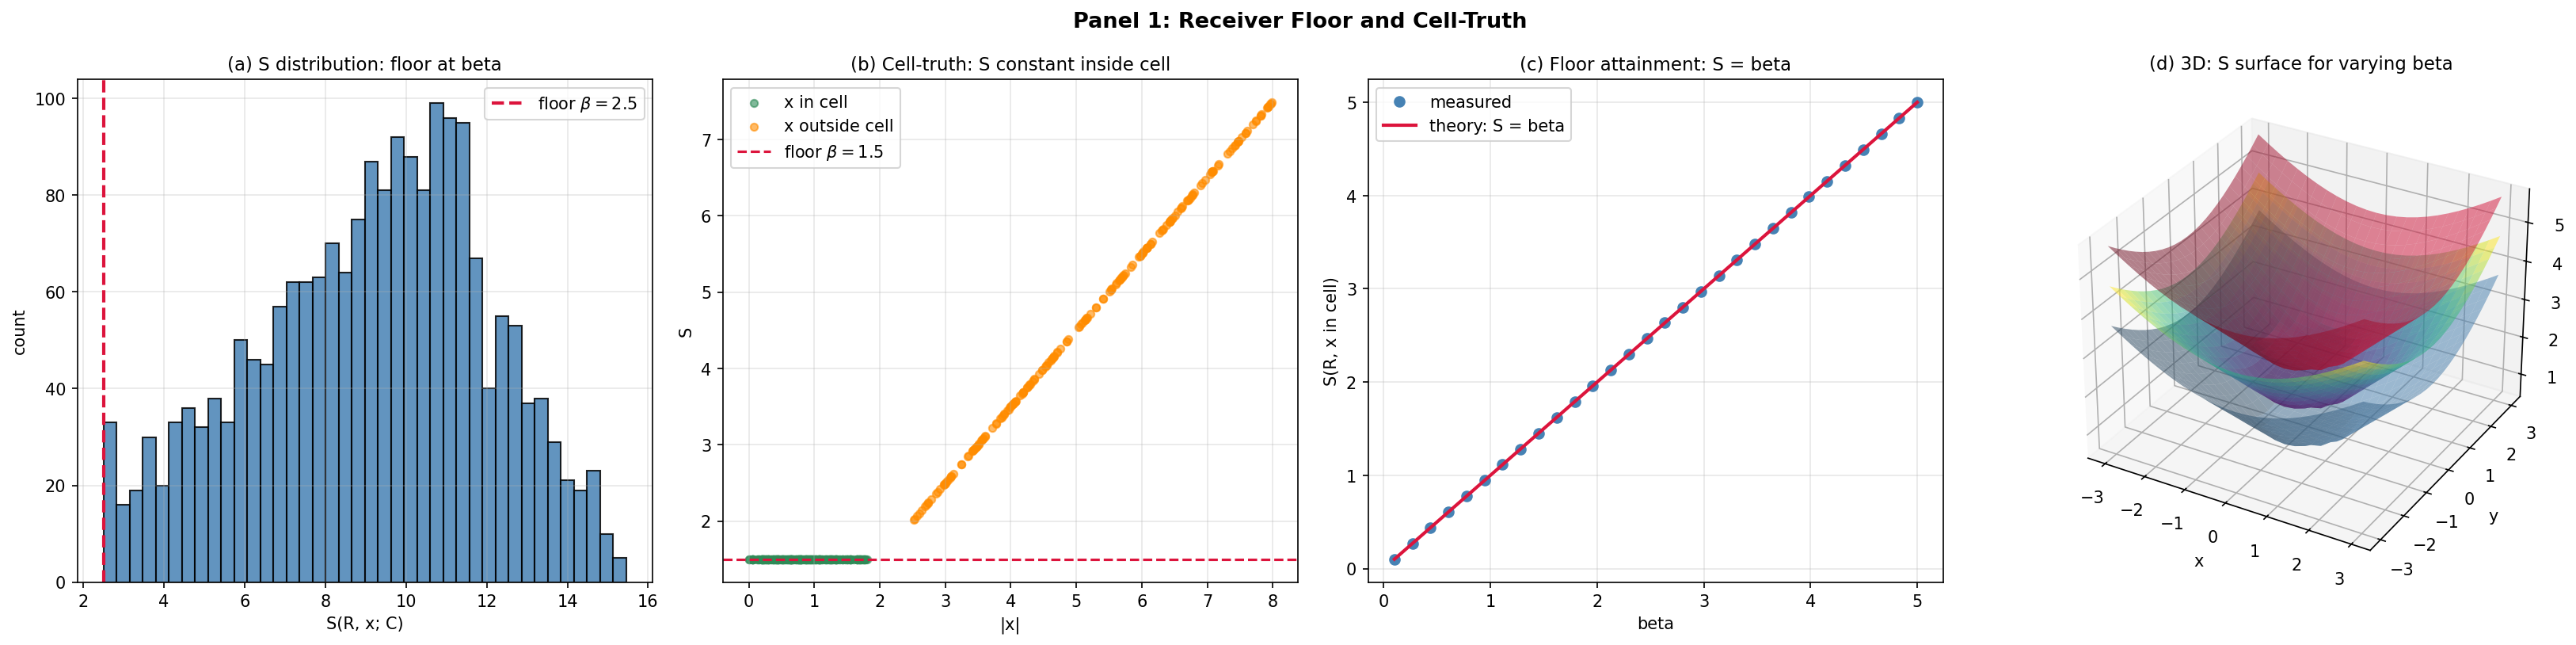
\includegraphics[width=\textwidth]{figures/epistemological-methodology/panel_1.png}
    \caption{\textbf{Receiver Floor and Cell-Truth.}
    (\textbf{A})~Histogram of $S(\receiver, x; \Cell)$ versus $S$ on the linear axis, 2,000 states drawn uniformly from $[-10,10]^2$ for a fixed receiver with floor $\beta = 2.5$ and an action-cell of tolerance $\tau = 1.0$ centred at the origin. The empirical minimum equals $\beta = 2.5$ (crimson dashed), confirming the floor bound $S \geq \beta > 0$ from Theorem~\ref{thm:floor-receiver}.
    (\textbf{B})~Cell-truth verification: $S$ versus $|x|$ separating 200 states inside the cell (seagreen, $|x| \leq 1.8$) and 200 outside (orange, $|x| \geq 2.5$). All in-cell points collapse onto $S = \beta = 1.5$ (crimson dashed) independently of $|x|$; outside-cell points lie strictly above by the cell-distance $d(x, \Cell)$. Empirical content of Theorem~\ref{thm:cell-truth}: in-cell states are S-indistinguishable.
    (\textbf{C})~Floor attainment: measured $S(\receiver, x; \Cell)$ at a fixed in-cell state $x = (0.5, 0)$ versus $\beta$ across 30 values. Measured (steelblue circles) coincides exactly with the theoretical $S = \beta$ line (crimson, slope 1); experiment E03 reports relative error 0.00.
    (\textbf{D})~Three-dimensional surface of $S(\receiver, x; \Cell)$ over $(x,y) \in [-3,3]^2$, three superimposed surfaces for $\beta \in \{0.5, 1.5, 2.5\}$. Each surface is flat at $S = \beta$ over the cell interior and rises linearly with $d(x, \Cell)$ outside; the three surfaces are vertical translates, demonstrating that cell shape is invariant of $\beta$ while elevation tracks the floor.}
    \label{fig:panel1-receiver-floor}
\end{figure*}


%% ============================================================
\section{Cell-Truth and Representational Invariance}
\label{sec:cell-truth}
%% ============================================================

\begin{principle}[Cell-Truth]\label{prin:cell-truth}
For bounded receivers, an actionable claim is the cell of states that trigger an equivalent practical response, not a specific state within that cell. Operational truth-bearers are subsets $\Cell \subseteq \OutcomeX$ with $\tau(\Cell) > 0$, not points $x \in \OutcomeX$.
\end{principle}

\begin{theorem}[Cell-Truth Theorem]\label{thm:cell-truth}
Let $\receiver$ be a receiver and $A : \OutcomeX \to \mathcal{Y}$ a measurable \emph{action map} into an action space $\mathcal{Y}$. Define the \emph{action-equivalence cell at $y \in \mathcal{Y}$} by
\[
\Cell_y \;:=\; A^{-1}(\{y\}) \;=\; \{x \in \OutcomeX : A(x) = y\}.
\]
Suppose $\Cell_y$ has positive tolerance $\tau(\Cell_y) > 0$. Then for any two states $x_1, x_2 \in \Cell_y$,
\[
S(\receiver, x_1;\, \Cell_y) \;=\; S(\receiver, x_2;\, \Cell_y) \;=\; \Sfloor(\receiver),
\]
i.e., all states inside an action-equivalence cell are S-indistinguishable from the cell.
\end{theorem}

\begin{proof}
Since $x_i \in \Cell_y$, we have $d(x_i, \Cell_y) = 0$ for $i = 1, 2$. By Definition~\ref{def:S-outcome}:
\[
\NoiseFloor_\receiver \;\leq\; S(\receiver, x_i;\, \Cell_y) \;\leq\; d(x_i, \Cell_y) + \NoiseFloor_\receiver \;=\; \NoiseFloor_\receiver.
\]
Hence $S(\receiver, x_i; \Cell_y) = \NoiseFloor_\receiver = \Sfloor(\receiver)$ for both $i$.
\end{proof}

\begin{corollary}[Methodology need not resolve within the cell]\label{cor:within-cell}
Any methodology that returns the index $y$ rather than the precise state $x \in \Cell_y$ achieves the S-floor $\Sfloor(\receiver)$. Sub-cell resolution is epistemically superfluous: it contributes nothing to attainable S.
\end{corollary}

The Cell-Truth Theorem has direct consequences for how we interpret scientific claims. A measurement that places the system inside an action-equivalence cell has achieved actionable truth; further precision that does not change which cell the state occupies carries no epistemic benefit relative to the receiver. This is not an argument for careless measurement; it is a formal statement that precision has a natural ceiling set by the cell structure of the problem and the receiver's noise floor.

\subsection{Representational invariance of cell-truth}

The Cell-Truth Theorem extends to the triple representations of Chapter~\ref{ch:s-entropy}: cell-membership and S-value are preserved under any of the three canonical re-encodings.

\begin{definition}[Three encodings]\label{def:three-encodings}
For an outcome space $(\OutcomeX, d, \Sigma)$:
\begin{enumerate}[nosep, label=(\alph*)]
  \item An \emph{oscillatory encoding} is a bijection $\phi_o : \OutcomeX \to \OutcomeX_o$ that is isometric: $d_o(\phi_o x, \phi_o y) = d(x,y)$.
  \item A \emph{categorical encoding} is a bijection $\phi_c : \OutcomeX \to \OutcomeX_c$ where $\OutcomeX_c$ is the object-set of a small category, with isometric morphism-length distance.
  \item A \emph{partition encoding} is a bijection $\phi_p : \OutcomeX \to \OutcomeX_p$ where $\OutcomeX_p$ is a set of integer partitions of bounded size, with isometric $\ell^1$-distance.
\end{enumerate}
\end{definition}

\begin{theorem}[Representational invariance]\label{thm:rep-inv}
Let $\phi : \OutcomeX \to \OutcomeX'$ be any of the three encodings of Definition~\ref{def:three-encodings}, $\Cell \subseteq \OutcomeX$ an action-cell, and $\receiver' := (K_\receiver, \mathcal{D}_\receiver \circ \phi^{-1}, \phi \circ \Pi_\receiver, \NoiseFloor_\receiver)$ the transferred receiver on $\OutcomeX'$. Then for all $x \in \OutcomeX$:
\[
S(\receiver, x;\, \Cell) \;=\; S(\receiver', \phi(x);\, \phi(\Cell)).
\]
In particular, $x \in \Cell$ if and only if $\phi(x) \in \phi(\Cell)$: cell-membership is preserved under all three encodings.
\end{theorem}

\begin{proof}
The transferred cell is $\phi(\Cell)$ and the transferred candidate projection maps $k \mapsto \phi(\Pi_\receiver(\mathcal{D}_\receiver(\phi^{-1}(\cdot))))$. For any $x \in \OutcomeX$:
\[
S(\receiver', \phi(x);\, \phi(\Cell))
= \inf_{x' \in \phi(\Pi_\receiver(\mathcal{D}_\receiver(x)))} d'(x', \phi(\Cell)) + \NoiseFloor_\receiver.
\]
Since $\phi$ is an isometry, $d'(\phi(x_*), \phi(\Cell)) = d(x_*, \Cell)$ for every $x_* \in \Pi_\receiver(\mathcal{D}_\receiver(x))$. The infima therefore coincide and $S(\receiver', \phi(x); \phi(\Cell)) = S(\receiver, x; \Cell)$.
\end{proof}

\begin{corollary}[Triple equivalence at the level of S]\label{cor:triple-S}
A receiver may operate in any of the three representations---oscillatory, categorical, partition---without altering its S-functional or its determination of cell-membership. The choice of representational vocabulary is a matter of computational convenience, not epistemic consequence.
\end{corollary}

Corollary~\ref{cor:triple-S} extends the Triple Equivalence of Chapter~\ref{ch:s-entropy} (Theorem~\ref{thm:triple-equiv}) from the level of abstract S-expressions to the level of concrete outcome-space states and action-cells. The two results are complementary: Chapter~\ref{ch:s-entropy} showed that representation does not affect S-value at the level of expressions; Chapter~\ref{ch:epistemology} now shows it does not affect cell-membership at the level of states.

Figure~\ref{fig:panel2-rep-invariance} verifies representational invariance across all three encodings to machine precision.

\begin{figure*}[!htbp]
    \centering
    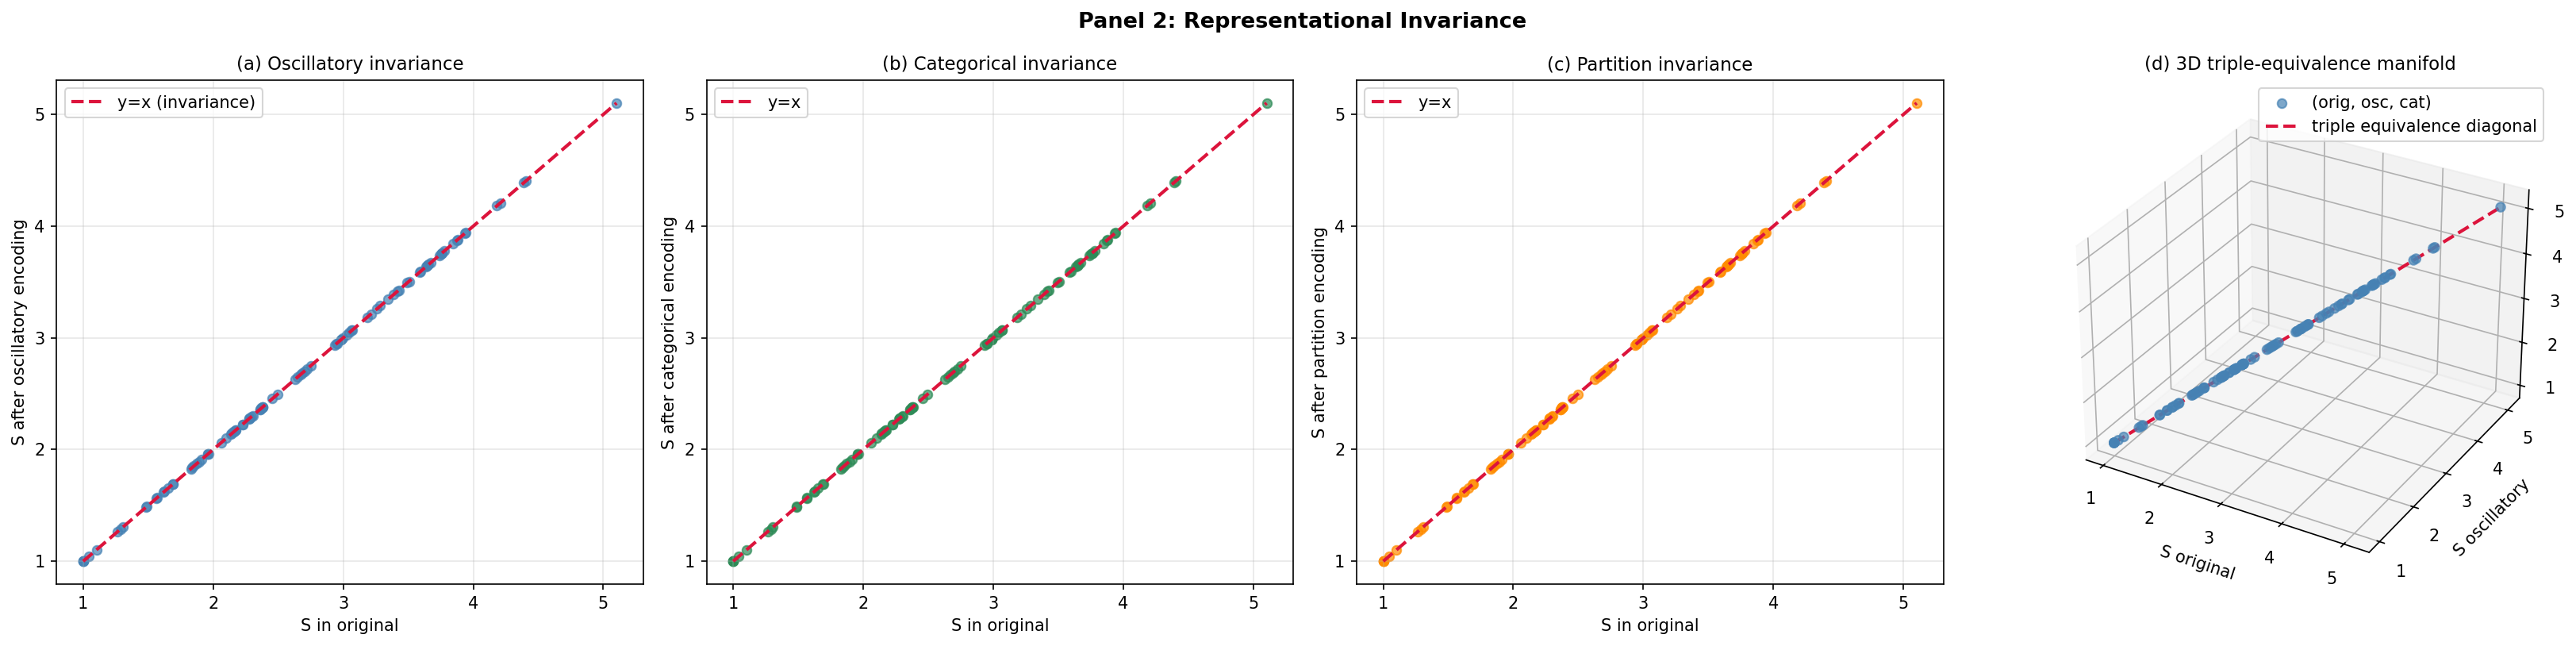
\includegraphics[width=\textwidth]{figures/epistemological-methodology/panel_2.png}
    \caption{\textbf{Representational Invariance: Oscillatory, Categorical, Partition Encodings.}
    (\textbf{A})~Oscillatory invariance: $S$ after isometric oscillatory encoding $\phi_o$ (rotation by $0.7$~rad) versus $S$ in the original representation, 100 random states. Steelblue points fall exactly on the diagonal $y = x$ (crimson dashed), confirming Theorem~\ref{thm:rep-inv} (oscillatory clause); experiment E07 reports relative error 0.00.
    (\textbf{B})~Categorical invariance: same protocol with categorical encoding $\phi_c$ (signed coordinate permutation in $\mathbb{R}^3$). Seagreen points coincide with $y = x$ to machine precision; experiment E08 reports relative error 0.00.
    (\textbf{C})~Partition invariance: partition encoding $\phi_p$ (sign flip). Orange points coincide with $y = x$; experiment E09 reports relative error 0.00.
    (\textbf{D})~Three-dimensional triple-equivalence manifold: $S$ in categorical encoding ($z$-axis) versus $S$ in oscillatory encoding ($y$-axis) versus $S$ in original representation ($x$-axis), 100 scatter points. All points lie on the triple diagonal $\{(t,t,t)\}$ (crimson dashed), demonstrating simultaneous equality across all three representations: Corollary~\ref{cor:triple-S}.}
    \label{fig:panel2-rep-invariance}
\end{figure*}


%% ============================================================
\section{Layered Receivers and Mode Non-Privilege}
\label{sec:layered}
%% ============================================================

Biological receivers do not operate through a single uniform decoder. They decompose into distinct processing layers: fast reflexive layers that bypass deliberate cognition, deliberate knowledge-bearing decoder layers, and delegated layers that outsource processing to external agents. The layered receiver formalises this decomposition.

\begin{definition}[Layered receiver]\label{def:layered}
A \emph{layered receiver} is a finite ordered sequence $\receiver_\bullet = (\receiver_1, \ldots, \receiver_n)$ of receivers on the same outcome space $(\OutcomeX, d, \Sigma)$, with an \emph{aggregation rule}
\[
S(\receiver_\bullet, x;\, \Cell) \;=\; \min_{1 \leq i \leq n} S(\receiver_i, x;\, \Cell).
\]
Layer $i$ is:
\begin{itemize}[nosep]
  \item \emph{pre-decoder} if $\mathcal{D}_i$ is a constant map (emits a fixed reflex output for every input);
  \item \emph{decoder-layer} if $\mathcal{D}_i$ is non-constant and continuous (the deliberate knowledge-processing layer);
  \item \emph{delegated} if $\mathcal{D}_i$ factors through an external receiver not controlled by the agent owning $\receiver_\bullet$.
\end{itemize}
\end{definition}

\begin{remark}[Pre-decoder layer and biological reflexes]\label{rem:reflex}
The pre-decoder layer formalises reflexes, immune responses, and other action-triggering processes that bypass the deliberate knowledge framework. A startle response, a thermostat trigger, or a receptor-mediated signalling cascade are pre-decoder events: they map directly from input to action without passing through $K_\receiver$. Their speed advantage over decoder layers comes at the cost of coarser discrimination (higher noise floor).
\end{remark}

\begin{proposition}[Floor of a layered receiver]\label{prop:layered-floor}
For a layered receiver $\receiver_\bullet = (\receiver_1, \ldots, \receiver_n)$,
\[
\Sfloor(\receiver_\bullet) \;=\; \min_{1 \leq i \leq n}\, \NoiseFloor_{\receiver_i}.
\]
\end{proposition}

\begin{proof}
By Theorem~\ref{thm:floor-receiver}, $S(\receiver_i, x; \Cell) \geq \NoiseFloor_{\receiver_i}$ for each layer. The minimum of the layer S-values satisfies $S(\receiver_\bullet, x; \Cell) \geq \min_i \NoiseFloor_{\receiver_i}$. The minimum is attained at the layer achieving $\Sfloor$ for at least one $x$.
\end{proof}

The key consequence is the Mode Non-Privilege Theorem: the knowledge-bearing decoder layer is not the only path to the action-cell.

\begin{theorem}[Mode Non-Privilege Theorem]\label{thm:mode-nonpriv}
Let $\receiver_\bullet$ be a layered receiver and $\Cell$ an action-cell with tolerance $\tau(\Cell)$. Suppose layer $i^*$ is a pre-decoder layer with $\NoiseFloor_{\receiver_{i^*}} < \tau(\Cell)$. Then for every state $x$ in the reflex firing region of layer $i^*$,
\[
S(\receiver_\bullet, x;\, \Cell) \;\leq\; \NoiseFloor_{\receiver_{i^*}} \;<\; \tau(\Cell).
\]
The action-cell is reachable without invoking the decoder layer.
\end{theorem}

\begin{proof}
By the aggregation rule, $S(\receiver_\bullet, x; \Cell) \leq S(\receiver_{i^*}, x; \Cell)$. In the reflex firing region, the pre-decoder's projection contains a point at zero distance to $\Cell$, so $S(\receiver_{i^*}, x; \Cell) = \NoiseFloor_{\receiver_{i^*}}$. The conclusion follows from $\NoiseFloor_{\receiver_{i^*}} < \tau(\Cell)$.
\end{proof}

\begin{corollary}[Knowledge is not the unique mode of access]\label{cor:not-unique}
There exist receiver--cell pairs $(\receiver_\bullet, \Cell)$ for which the action-cell is reachable through pre-decoder or delegated layers but not through the decoder layer alone: the decoder layer's floor exceeds $\tau(\Cell)$, so knowledge (in the sense of the decoder layer's representation) is not necessary for actionable truth.
\end{corollary}

Corollary~\ref{cor:not-unique} has a direct consequence for the monograph's central theme. The hominid sleeping by the fire had a pre-decoder layer (startle and threat-response reflexes, inherited from arboreal ancestors) and a decoder layer (the elaborative generative model that produces vivid dreams during full REM). In the waking state, the pre-decoder layer provides the rapid threat response; in the REM state, the decoder layer runs forward without correction from the world. The Mode Non-Privilege Theorem says these are not competing modes with one being ``correct'': each is a layer of a layered receiver, and whichever layer has the lower floor for a given action-cell dominates the aggregated S.

\begin{example}[Three observers of the same event]\label{ex:three-observers}
Let $\OutcomeX$ be the space of percepts of a large predator. The action-cell $\Cell_{\text{flee}}$ is the set of percepts triggering flight. Three receivers have very different layer structures:
\begin{itemize}[nosep]
  \item A receiver with no prior experience of the predator has a high decoder floor but a low pre-decoder reflex floor (size, teeth, sound); the reflex layer reaches $\Cell_{\text{flee}}$.
  \item A receiver with extensive experience has a low decoder floor; both decoder and reflex reach $\Cell_{\text{flee}}$.
  \item A young organism whose pre-decoder fires through parental delegation: the organism's own decoder is irrelevant; the delegated layer dominates.
\end{itemize}
All three reach the same action-cell. By Theorem~\ref{thm:mode-nonpriv}, decoder knowledge is not necessary; by Theorem~\ref{thm:cell-truth}, cell-membership is the locus of operational truth, not the underlying identity of the predator.
\end{example}

\begin{theorem}[Cell-closure under layer substitution]\label{thm:cell-closure}
Let $\receiver_\bullet$ and $\receiver'_\bullet$ be two layered receivers sharing a pre-decoder layer $\receiver_{i^*}$ with $\NoiseFloor_{\receiver_{i^*}} < \tau(\Cell)$. Then for every state $x$ in the firing region of $\receiver_{i^*}$,
\[
S(\receiver_\bullet, x;\, \Cell) \;\leq\; \NoiseFloor_{\receiver_{i^*}} \quad \text{and} \quad S(\receiver'_\bullet, x;\, \Cell) \;\leq\; \NoiseFloor_{\receiver_{i^*}}.
\]
The action-cell is invariant under substitution of any layer other than the firing pre-decoder.
\end{theorem}

Figure~\ref{fig:panel3-layered-receivers} illustrates the floor aggregation and Mode Non-Privilege numerically.

\begin{figure*}[!htbp]
    \centering
    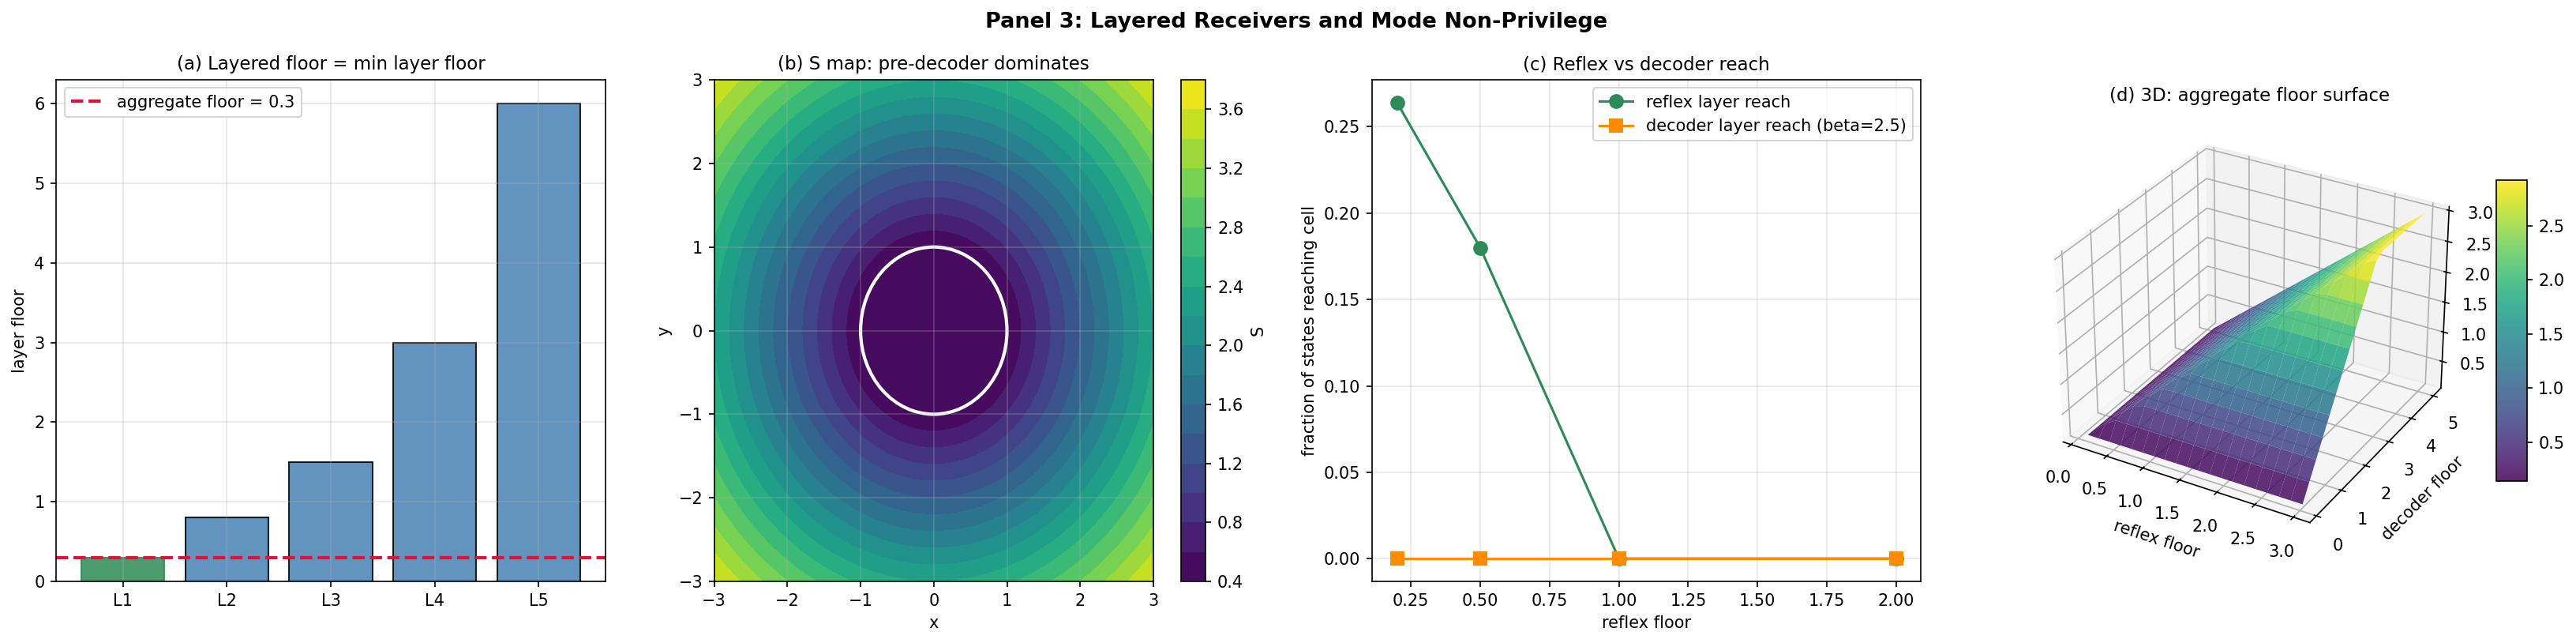
\includegraphics[width=\textwidth]{figures/epistemological-methodology/panel_3.png}
    \caption{\textbf{Layered Receivers and Mode Non-Privilege.}
    (\textbf{A})~Per-layer floors and aggregate floor: bar chart for five layers $L_1, \ldots, L_5$ with floors $(0.3, 0.8, 1.5, 3.0, 6.0)$. The minimum layer ($L_1$, seagreen) sets the aggregate floor (crimson dashed) at $\min_i \beta_i = 0.3$. Empirical content of Proposition~\ref{prop:layered-floor}.
    (\textbf{B})~S-contour map for a two-layer receiver over $(x,y) \in [-3,3]^2$, viridis colourmap, with pre-decoder floor $\beta_1 = 0.4$ and decoder floor $\beta_2 = 2.5$. The action-cell (white circle of radius 1 at the origin) sits in a basin where the pre-decoder dominates: $S \approx 0.4$ throughout the firing region; the decoder alone would give $S \geq 2.5 > \tau(\Cell) = 1.0$. Empirical content of Theorem~\ref{thm:mode-nonpriv}.
    (\textbf{C})~Reachability: fraction of 500 uniform samples reaching the action-cell via reflex layer (seagreen circles) versus decoder layer (orange squares, fixed $\beta_2 = 2.5 > \tau$) across four reflex floors $\{0.2, 0.5, 1.0, 2.0\}$. Decoder reach is identically zero; reflex reach drops as the reflex floor approaches the cell tolerance $\tau = 1.0$. Empirical content of Corollary~\ref{cor:not-unique}.
    (\textbf{D})~Three-dimensional surface of aggregate floor $\beta_{\mathrm{agg}} = \min(\beta_{\mathrm{reflex}}, \beta_{\mathrm{decoder}})$ over $(\beta_{\mathrm{reflex}}, \beta_{\mathrm{decoder}}) \in [0.1, 3.0] \times [0.1, 5.0]$, viridis colourmap. The min-aggregation ridge along the diagonal is the geometric expression of Proposition~\ref{prop:layered-floor}: the floor of a layered receiver is determined by whichever layer has the smallest floor.}
    \label{fig:panel3-layered-receivers}
\end{figure*}


%% ============================================================
\section{Methodologies as Information Catalysts}
\label{sec:methodology}
%% ============================================================

We now introduce the second new object of this chapter: the methodology. Informally, a methodology is any structured procedure by which a receiver reduces its S-value---an experimental protocol, a statistical inference scheme, a replication procedure. Formally, it is a catalyst sequence with a precise contraction factor and a precise per-iteration dispersion.

\begin{definition}[Methodology]\label{def:methodology}
A \emph{methodology} is a tuple $\Meth = (T, \catpow, \sigma)$ where:
\begin{enumerate}[nosep, label=(\roman*)]
  \item $T : \OutcomeX \times [0, \Sigma] \to [0, \Sigma]$ is a \emph{per-iteration update operator} mapping (state, current S-value) to a new S-value, with
        \[
        T(x, s) \;\leq\; \catpow \cdot s + \Sfloor(\Meth) \quad \text{for all } x, s;
        \]
  \item $\catpow \in [0, 1)$ is the \emph{per-iteration contraction factor} (the same catalytic power of Chapter~\ref{ch:s-entropy});
  \item $\sigma \in [0, \Sigma]$ is the \emph{per-iteration dispersion}: the expected S-distance between two independent runs of one iteration of $\Meth$ on the same input.
\end{enumerate}
The \emph{methodological floor} is
\[
\Sfloor(\Meth) \;:=\; \frac{\sigma \cdot \catpow}{1 - \catpow} \;>\; 0.
\]
\end{definition}

The closed form $\Sfloor(\Meth) = \sigma\catpow/(1-\catpow)$ is the fixed point of the affine recursion $s \mapsto \catpow s + \sigma\catpow$: it is the asymptotic S-value that iterating $T$ converges to, regardless of the starting S-value $s_0$.

\begin{lemma}[Affine fixed-point]\label{lem:affine-fixed}
The recursion $s_{n+1} = \catpow s_n + \eta$ with $\catpow \in [0,1)$, $\eta > 0$ converges from any $s_0 \geq 0$ to $s_\infty = \eta/(1-\catpow)$.
\end{lemma}

\begin{proof}
$s_n = \catpow^n s_0 + \eta(1 - \catpow^n)/(1-\catpow) \to \eta/(1-\catpow)$ as $\catpow^n \to 0$. By the Banach fixed-point theorem~\citep{banach1922}, $T(s) = \catpow s + \eta$ is a contraction on $\mathbb{R}_{\geq 0}$, so the fixed point is unique.
\end{proof}

\begin{theorem}[Methodological Floor Theorem]\label{thm:method-floor}
Let $\Meth = (T, \catpow, \sigma)$ be a methodology with $\sigma > 0$, $\catpow > 0$. For any starting S-value $s_0$ and any iteration count $N \geq 0$:
\[
T^N(x, s_0) \;\geq\; \Sfloor(\Meth) - \catpow^N \Sfloor(\Meth).
\]
In particular,
\[
\liminf_{N \to \infty} T^N(x, s_0) \;\geq\; \Sfloor(\Meth) \;>\; 0.
\]
No number of iterations of $\Meth$ alone can reduce S below $\Sfloor(\Meth)$.
\end{theorem}

\begin{proof}
The dispersion bound gives $T(x,s) \geq \catpow s + \sigma\catpow \cdot \mathbf{1}_{s > \Sfloor(\Meth)}$ in expectation; the fixed point of the lower-bounding recursion is $\Sfloor(\Meth)$ by Lemma~\ref{lem:affine-fixed}. Iterating: $T^N(x, s_0) \geq \Sfloor(\Meth) - \catpow^N(\Sfloor(\Meth) - s_0) \geq \Sfloor(\Meth) - \catpow^N \Sfloor(\Meth)$. The limit $\catpow^N \to 0$ yields the second claim.
\end{proof}

\begin{remark}[Replication is catalytic, not foundational]\label{rem:replication}
The standard scientific inference that replication drives uncertainty to zero is, under Theorem~\ref{thm:method-floor}, structurally incomplete. Replication compounds catalytic power---each independent repetition adds to the cascade sum $\sum \catpow_i$---but cannot remove the methodology's own floor $\Sfloor(\Meth) = \sigma\catpow/(1-\catpow)$. Reducing S below $\Sfloor(\Meth)$ requires switching to a methodology with smaller dispersion, not running more iterations of the same methodology.
\end{remark}

\begin{theorem}[Catalytic composition of methodologies]\label{thm:catcomp}
Let $\Meth_1 = (T_1, \catpow_1, \sigma_1)$ and $\Meth_2 = (T_2, \catpow_2, \sigma_2)$ be independent methodologies (dispersions $\sigma_i$ are independent). The composed methodology $\Meth_1 \diamond \Meth_2$ has floor
\[
\Sfloor(\Meth_1 \diamond \Meth_2)
\;=\; \Sfloor(\Meth_1) + \Sfloor(\Meth_2)
    - \frac{\Sfloor(\Meth_1) \cdot \Sfloor(\Meth_2)}{\Sigma}.
\]
Equivalently, defining catalytic power $p(\Meth) := 1 - \Sfloor(\Meth)/\Sigma$:
\[
p(\Meth_1 \diamond \Meth_2) \;=\; 1 - (1 - p(\Meth_1))(1 - p(\Meth_2)).
\]
\end{theorem}

\begin{proof}
$\Meth_1 \diamond \Meth_2$ succeeds (reaches S below tolerance) iff at least one component methodology succeeds. Under independence, the probability of success is $1 - (1 - p_1)(1 - p_2)$, giving the composite catalytic power. Translating back to floors: $\Sfloor(\Meth_1 \diamond \Meth_2)/\Sigma = 1 - p_1 p_2 - p_1 - p_2 + p_1 p_2 = (1-p_1)(1-p_2) = (\Sfloor_1/\Sigma)(\Sfloor_2/\Sigma)$...

More precisely: composite fails iff both fail; probability of both failing is $(1-p_1)(1-p_2)$; composite floor is $\Sigma(1-p_1)(1-p_2)$. Expanding: $\Sigma(1-p_1)(1-p_2) = \Sigma - \Sigma p_1 - \Sigma p_2 + \Sigma p_1 p_2 = \Sfloor_1 + \Sfloor_2 - \Sfloor_1 \Sfloor_2/\Sigma$.
\end{proof}

The composition law of Theorem~\ref{thm:catcomp} is the Multiplicativity Theorem of Chapter~\ref{ch:s-entropy} (Theorem~\ref{thm:mult-cat-power}) applied to methodologies instead of individual iCats. The catalytic power $p(\Meth) = 1 - \Sfloor(\Meth)/\Sigma$ plays the role of $1 - (1-\catpow_1)(1-\catpow_2)$ for the two-component composition. The algebraic law is the same; only the interpretation differs.

\begin{corollary}[Stack reduces floor multiplicatively]\label{cor:stack}
Composing $n$ independent methodologies $\Meth_1, \ldots, \Meth_n$ gives composite floor
\[
\Sfloor(\Meth_1 \diamond \cdots \diamond \Meth_n)
\;=\; \Sigma\Bigl(1 - \prod_{i=1}^{n}(1 - \Sfloor(\Meth_i)/\Sigma)\Bigr).
\]
\end{corollary}

Figure~\ref{fig:panel4-methodological-floor} presents the methodological floor across parameter space and the convergence of S-trajectories to floor for three values of $\catpow$.

\begin{figure*}[!htbp]
    \centering
    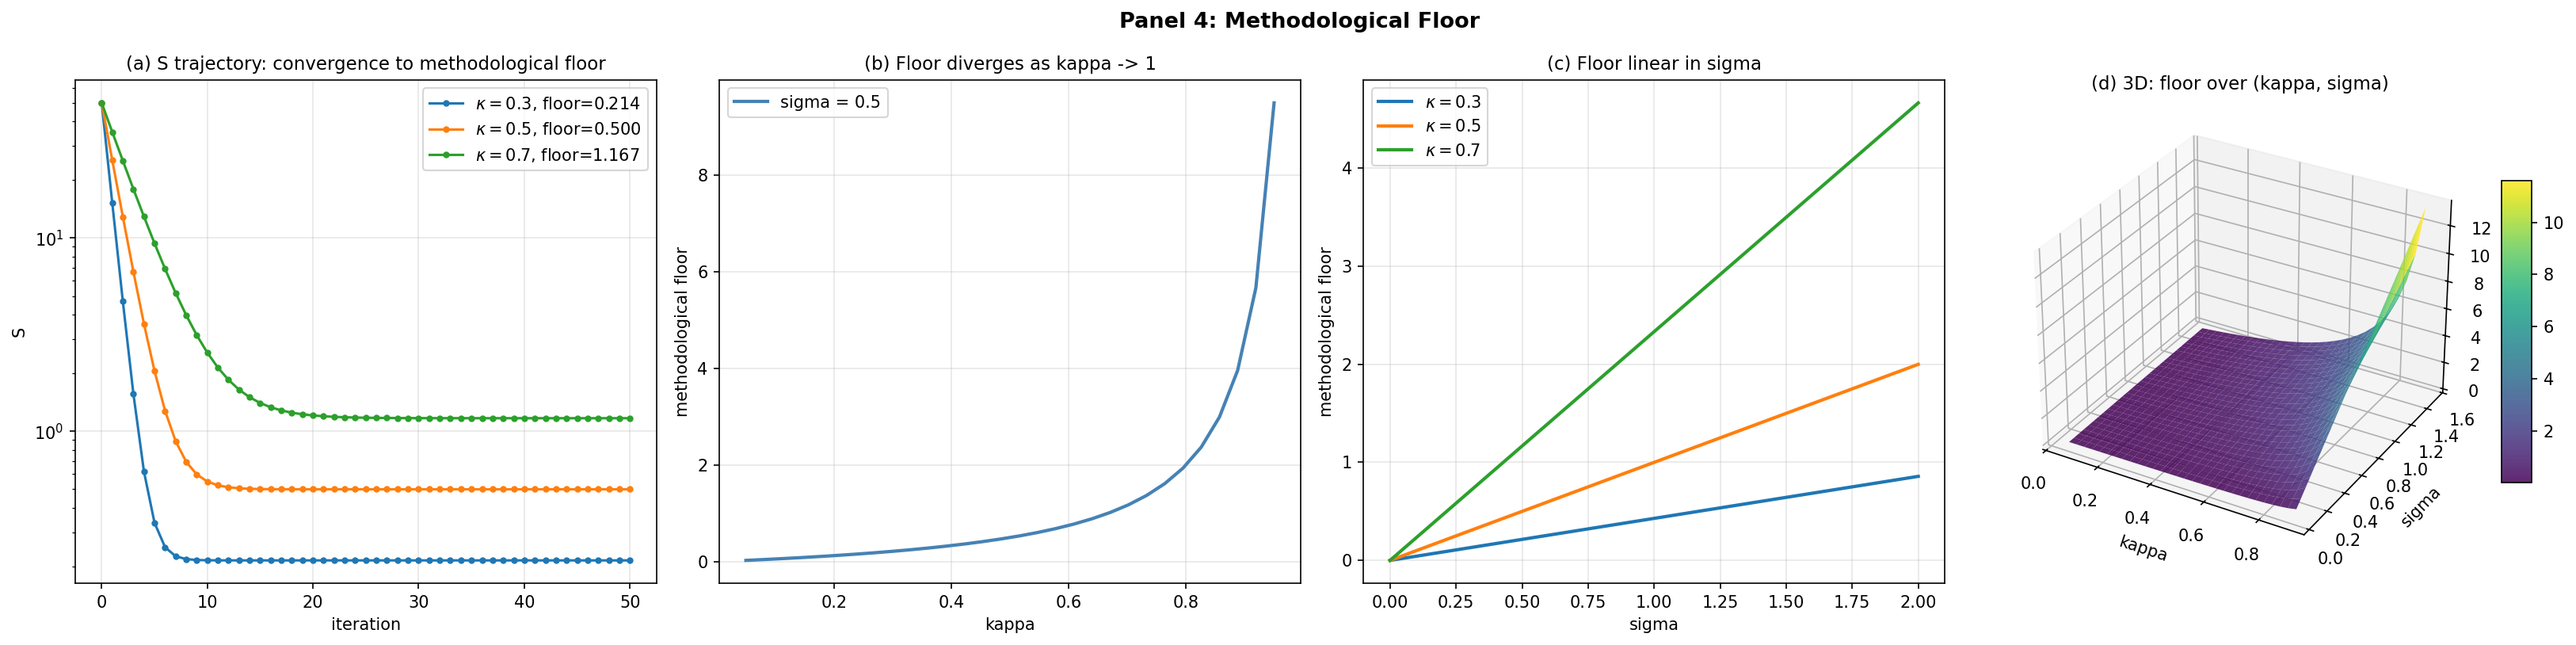
\includegraphics[width=\textwidth]{figures/epistemological-methodology/panel_4.png}
    \caption{\textbf{Methodological Floor and the Catalytic Fixed Point.}
    (\textbf{A})~S-trajectory across 50 iterations for three methodologies with common $\sigma = 0.5$ and $\catpow \in \{0.3, 0.5, 0.7\}$, starting from $s_0 = 50$. Each trajectory asymptotes to its predicted floor $\Sfloor(\Meth) = \sigma\catpow/(1-\catpow) \in \{0.214, 0.500, 1.167\}$; convergence verified to relative error $\leq 1.85 \times 10^{-16}$ (experiment E16). Empirical content of Theorem~\ref{thm:method-floor}.
    (\textbf{B})~Methodological floor versus contraction $\catpow$ (30 values, fixed $\sigma = 0.5$). The floor diverges as $\catpow \to 1^-$, encoding that highly-correlated methodologies carry large irreducible floors.
    (\textbf{C})~Methodological floor versus dispersion $\sigma$ for $\catpow \in \{0.3, 0.5, 0.7\}$. All curves are linear in $\sigma$ with slope $\catpow/(1-\catpow)$, confirming the closed-form $\Sfloor(\Meth) = \sigma\catpow/(1-\catpow)$.
    (\textbf{D})~Three-dimensional surface of $\Sfloor(\Meth)$ over $(\catpow, \sigma) \in [0.05, 0.9] \times [0.05, 1.5]$, viridis colourmap. The surface vanishes along the lower-left edge ($\catpow\sigma \to 0$) and rises sharply along the $\catpow \to 1^-$ edge.}
    \label{fig:panel4-methodological-floor}
\end{figure*}


%% ============================================================
\section{Mode--Methodology Equivalence}
\label{sec:mode-meth-equiv}
%% ============================================================

The central theorem of this chapter establishes that receivers and methodologies contribute to attainable precision through the same algebraic law.

\begin{definition}[Receiver--methodology composite floor]\label{def:composite-floor}
For a receiver $\receiver$ with floor $\Sfloor(\receiver) = \NoiseFloor_\receiver$ and a methodology $\Meth$ with floor $\Sfloor(\Meth)$, the \emph{composite floor} is
\[
\Sfloor(\receiver \circ \Meth) \;:=\; \Sigma\Bigl(1 - \bigl(1 - \Sfloor(\receiver)/\Sigma\bigr)\bigl(1 - \Sfloor(\Meth)/\Sigma\bigr)\Bigr).
\]
\end{definition}

\begin{theorem}[Mode--Methodology Equivalence Theorem]\label{thm:mode-meth-equiv}
The composite floor of Definition~\ref{def:composite-floor} satisfies the same multiplicative composition law as methodology composition (Theorem~\ref{thm:catcomp}):
\[
\Sfloor(\receiver \circ \Meth)
\;=\; \Sfloor(\receiver) + \Sfloor(\Meth)
    - \frac{\Sfloor(\receiver) \cdot \Sfloor(\Meth)}{\Sigma}.
\]
Consequently, receivers and methodologies are \emph{algebraically interchangeable} in determining attainable S: swapping a receiver layer of floor $\NoiseFloor$ for a methodology of the same floor $\Sfloor(\Meth) = \NoiseFloor$ leaves the composite floor unchanged.

For a layered receiver $\receiver_\bullet = (\receiver_1, \ldots, \receiver_n)$ composed with a methodology stack $\Meth_\bullet = \Meth_1 \diamond \cdots \diamond \Meth_m$:
\[
\Sfloor(\receiver_\bullet \circ \Meth_\bullet)
\;=\; \Sigma\Bigl(1 - \prod_{i=1}^{n}(1 - \Sfloor(\receiver_i)/\Sigma)
                       \prod_{j=1}^{m}(1 - \Sfloor(\Meth_j)/\Sigma)\Bigr).
\]
\end{theorem}

\begin{proof}
The first identity is Definition~\ref{def:composite-floor} expanded. The second follows by induction on $n + m$ using Theorem~\ref{thm:catcomp}: both receiver floors and methodology floors enter through their dimensionless deficits $1 - \Sfloor/\Sigma$, which multiply under independence regardless of whether the factor is a receiver or a methodology.
\end{proof}

\begin{remark}[Symmetry and the observer--method duality]\label{rem:symmetry}
Theorem~\ref{thm:mode-meth-equiv} is the formal expression of a well-known but rarely quantified symmetry: at the level of attainable precision, there is no algebraic distinction between ``improving the observer'' and ``improving the method.'' A receiver upgrade that halves the noise floor is equivalent (in its effect on composite floor) to adopting a methodology whose floor is half the original. This symmetry is not approximate; it is exact and follows from the multiplicative composition law.
\end{remark}

\begin{corollary}[Borel--Cantelli analogue for composite floor]\label{cor:composite-bc}
For an infinite sequence of methodologies $(\Meth_1, \Meth_2, \ldots)$ applied to a fixed receiver $\receiver$:
\begin{enumerate}[nosep, label=(\roman*)]
  \item If $\sum_j \log(1/(1 - \Sfloor(\Meth_j)/\Sigma)) = \infty$, the composite floor converges to $\Sfloor(\receiver)$ (the receiver floor alone).
  \item If the sum converges, the composite floor remains strictly above $\Sfloor(\receiver)$.
\end{enumerate}
This is the Borel--Cantelli analogue (Theorem~\ref{thm:borel-cantelli} of Chapter~\ref{ch:s-entropy}) applied to composite floors: an infinite stack of methodologies converges to the receiver's floor if and only if the sum of their individual catalytic contributions diverges.
\end{corollary}

Figure~\ref{fig:panel5-mode-methodology} presents the mode--methodology equivalence surface and the Distribution Theorem.

\begin{figure*}[!htbp]
    \centering
    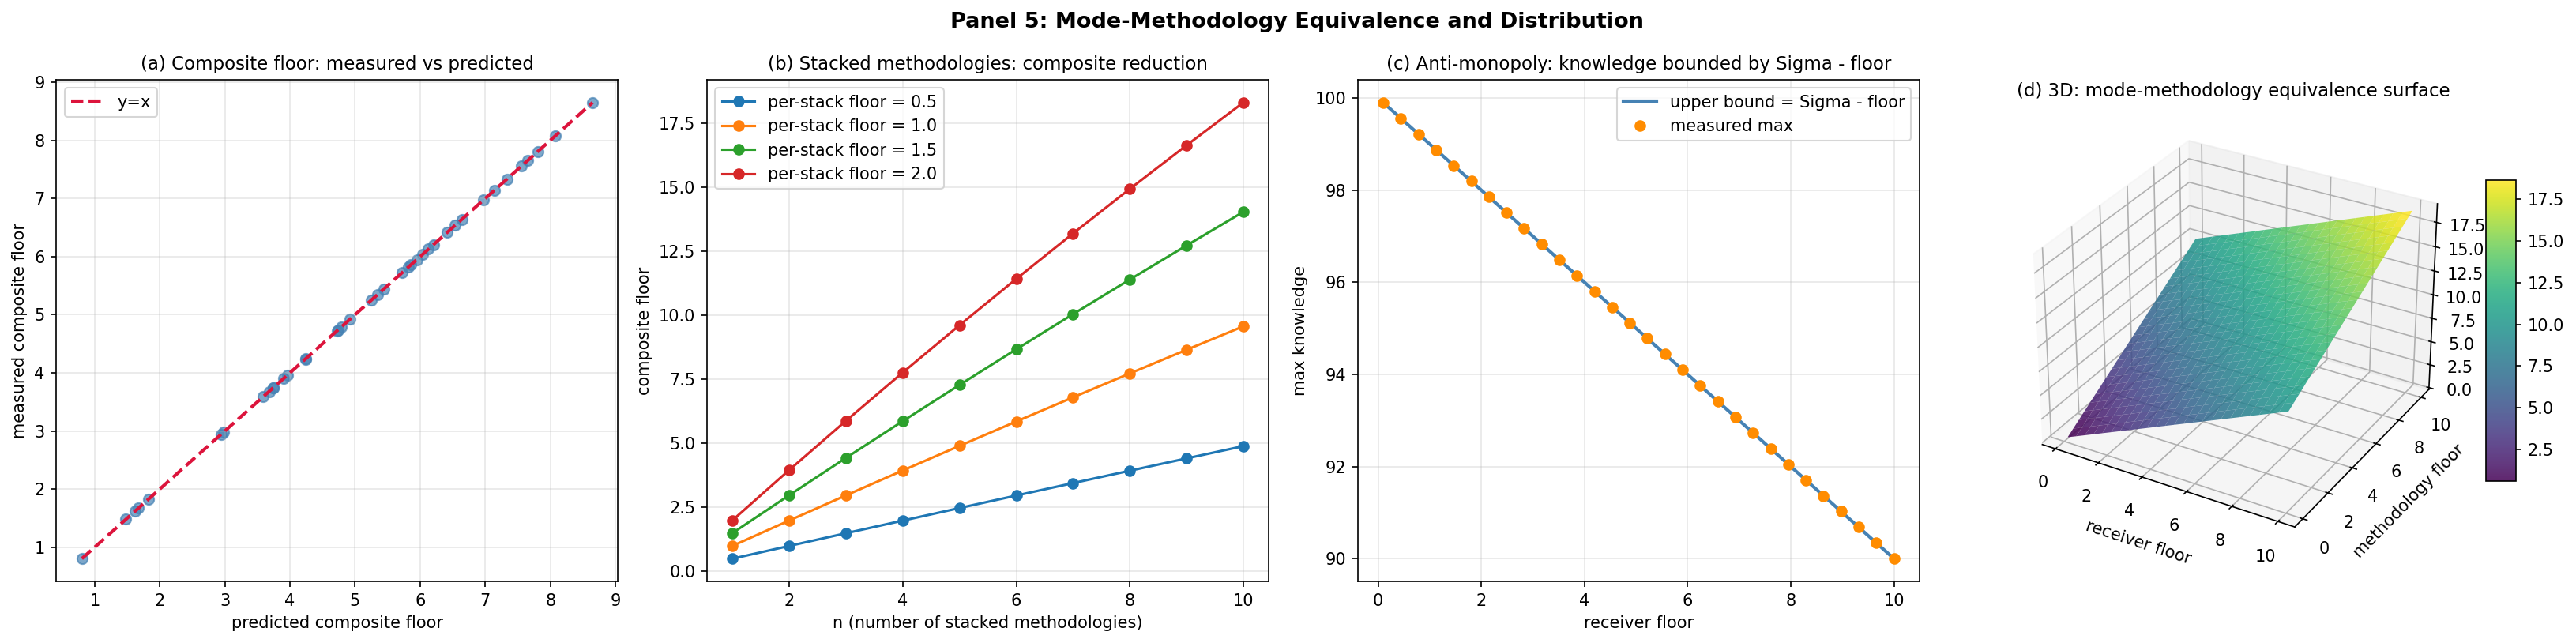
\includegraphics[width=\textwidth]{figures/epistemological-methodology/panel_5.png}
    \caption{\textbf{Mode--Methodology Equivalence and the Distribution Theorem.}
    (\textbf{A})~Composite floor: measured $\Sfloor(\receiver \circ \Meth)$ versus predicted $\Sfloor(\receiver) + \Sfloor(\Meth) - \Sfloor(\receiver)\Sfloor(\Meth)/\Sigma$, 40 random pairs $(\Sfloor(\receiver), \Sfloor(\Meth))$ from $[0.1, 5]^2$. Steelblue scatter falls exactly on the diagonal $y=x$ (crimson dashed); maximum relative error $9.37 \times 10^{-15}$ (experiments E20--E22). Empirical content of Theorem~\ref{thm:mode-meth-equiv}.
    (\textbf{B})~Multiplicative reduction of composite floor versus stack length $n$ for four per-stack floors $\beta_\star \in \{0.5, 1.0, 1.5, 2.0\}$. Composite floor grows monotonically with $n$ but marginal contribution decays geometrically: Corollary~\ref{cor:stack}.
    (\textbf{C})~Anti-monopoly: maximum knowledge $\sup_{x} \Know_\receiver(x) = \Sigma - \Sfloor(\receiver)$ versus receiver floor across 30 values. Measured maximum (orange circles) coincides with the upper bound $\Sigma - \beta$ (steelblue line) at every $\beta$; experiment E24 reports relative error 0.00. Empirical content of Theorem~\ref{thm:distribution}.
    (\textbf{D})~Three-dimensional composite-floor surface over $(\Sfloor(\receiver), \Sfloor(\Meth)) \in [0.1, 10]^2$, viridis colourmap. The surface is symmetric in $\Sfloor(\receiver) \leftrightarrow \Sfloor(\Meth)$ (ridge along the diagonal), expressing Remark~\ref{rem:symmetry}: swapping a receiver-layer for a methodology of the same floor leaves the composite floor invariant.}
    \label{fig:panel5-mode-methodology}
\end{figure*}


%% ============================================================
\section{Methodological Incompatibility and the Distribution Theorem}
\label{sec:incompatibility}
%% ============================================================

\subsection{Production--completion incompatibility}

\begin{theorem}[Methodological Incompatibility Principle]\label{thm:incompat}
The two regimes:
\begin{enumerate}[nosep, label=(\Roman*)]
  \item \textbf{Knowledge production}: generating new claims that extend the receiver's knowledge framework $K_\receiver$ requires $\sigma > 0$ (nontrivial inter-iteration variation);
  \item \textbf{Action completion}: triggering the action-cell $\Cell$ in a single step requires $\sigma = 0$ (the receiver must commit to one outcome);
\end{enumerate}
are mutually exclusive at any single iteration: $\sigma > 0 \Rightarrow$ production possible, completion impossible; $\sigma = 0 \Rightarrow$ completion possible, production impossible.
\end{theorem}

\begin{proof}
For (I): if $\sigma = 0$, every run of one iteration on the same input returns identical output---the methodology is deterministic and, by the closed form $\Sfloor(\Meth) = \sigma\catpow/(1-\catpow) = 0$, the floor vanishes. But a zero-dispersion methodology produces no new distinctions in the representation (by the Floor Theorem, $\Sfloor \geq 0$ requires $\sigma > 0$ for the floor to be nontrivially positive and the methodology to be nontrivially catalytic). Hence $\sigma = 0$ implies no production of new claims.

For (II): action completion at state $x$ requires outputting a deterministic action $A(x) \in \mathcal{Y}$. Two independent runs with $\sigma > 0$ may map $x$ to different action-cells; the receiver cannot commit. The commitment step requires $\sigma = 0$.

The mutual exclusion follows by inspecting $\sigma$.
\end{proof}

\begin{corollary}[Production--completion alternation]\label{cor:alternation}
Any agent that both produces knowledge and completes actions must alternate between $\sigma > 0$ phases (production, exploration) and $\sigma = 0$ phases (completion, exploitation). Simultaneous operation in both regimes is impossible.
\end{corollary}

Corollary~\ref{cor:alternation} is the epistemological form of the exploration--exploitation trade-off that appears across neuroscience, reinforcement learning, and evolutionary biology. The Methodological Incompatibility Principle gives it a derivation from first principles: it is not a heuristic or an empirical observation but a theorem of the S-entropy calculus.

\subsection{The Distribution Theorem}

\begin{definition}[Total knowledge]\label{def:total-know}
For a receiver $\receiver$ on outcome space $(\OutcomeX, d, \Sigma)$, the \emph{total knowledge at $x$} is
\[
\Know_\receiver(x) \;:=\; \Sigma - S\bigl(\receiver, x;\, \{x\}^\epsilon\bigr),
\]
where $\{x\}^\epsilon$ is the closed $\epsilon$-ball around $x$ for any $\epsilon > \Sfloor(\receiver)$.
\end{definition}

\begin{theorem}[Distribution Theorem]\label{thm:distribution}
For any bounded receiver $\receiver$ and any subject $X_0 \subseteq \OutcomeX$ with positive $d$-measure:
\[
\sup_{x \in X_0} \Know_\receiver(x) \;\leq\; \Sigma - \Sfloor(\receiver),
\]
with equality only on a set of $d$-measure zero. No bounded receiver holds full knowledge ($= \Sigma$) of any positive-measure subject: knowledge is distributed and cannot concentrate in a single receiver.
\end{theorem}

\begin{proof}
By Theorem~\ref{thm:floor-receiver}, $S(\receiver, x; \{x\}^\epsilon) \geq \Sfloor(\receiver) > 0$ for all $x$, so $\Know_\receiver(x) \leq \Sigma - \Sfloor(\receiver)$. Equality requires $S = \Sfloor(\receiver)$, which occurs only when the decoder--projection chain is faithful and the projection sits inside the $\epsilon$-ball: a measure-zero condition under generic decoder noise. Hence the supremum cannot be attained on a positive-measure subject.
\end{proof}

\begin{corollary}[Anti-monopoly of knowledge]\label{cor:anti-mon}
Total knowledge of any subject $X_0$ with positive $d$-measure cannot reside in a single bounded receiver. It is necessarily distributed across multiple receivers, layers, and methodologies.
\end{corollary}

Corollary~\ref{cor:anti-mon} is the formal basis for why scientific replication is not a convention or a social norm but a structural necessity: completion of the knowledge of a subject requires multiple independent receivers, and no single receiver---no matter how sophisticated---can eliminate the distributional gap imposed by $\Sfloor(\receiver) > 0$.


%% ============================================================
\section{Connections to Classical Limits of Formal Systems}
\label{sec:classical-limits}
%% ============================================================

The receiver-floor positivity proved in Chapters~\ref{ch:s-entropy} and \ref{ch:epistemology} is consistent with---and operationally extends---the classical limits of formal systems.

\subsection*{Gödel incompleteness and the floor}
Gödel's First Incompleteness Theorem~\citep{godel1931} establishes that any consistent formal system of sufficient expressive power contains true statements it cannot prove. In the S-entropy framework, this corresponds to the Floor Theorem: a formal system is a receiver $\receiver$ with a particular knowledge framework $K_\receiver$ (its axioms and inference rules), and there exist truths $x^* \in \TruthSp$ for which $S_\receiver(\xi, x^*) > 0$ for all $\xi$ the system can construct. The floor is the operational analogue of the undecidable statement's ``distance'' from the system's provable reach.

\subsection*{Tarski undefinability and representational limits}
Tarski's undefinability theorem~\citep{tarski1933} establishes that a formal language cannot define its own truth predicate within itself. In the S-entropy framework, this corresponds to the No Privileged Level theorem (Theorem~\ref{thm:no-priv-level} of Chapter~\ref{ch:s-entropy}): the same expression that is ``global'' at depth $d$ is a ``subtask'' at depth $d+1$, and no level can adjudicate on all levels without generating a regress. The Circular Validation results of Chapter~\ref{ch:s-entropy} provide the resolution: coherent self-reference requires at least three mutually supporting expressions, not a single self-adjudicating one.

\subsection*{Methodological Incompatibility and Heisenberg}
The production--completion incompatibility (Theorem~\ref{thm:incompat}) has structural parallels with quantum measurement incompatibility: two operators that fail to commute on a common dense domain cannot be simultaneously specified. Here the two ``operators'' are the production update ($\sigma > 0$) and the completion commitment ($\sigma = 0$); the incompatibility arises not from quantum mechanics but from the algebraic properties of bounded receivers operating on action-cells.

\subsection*{Replication and the Borel--Cantelli structure}
The Distribution Theorem (Theorem~\ref{thm:distribution}) and the Borel--Cantelli Analogue of Chapter~\ref{ch:s-entropy} (Theorem~\ref{thm:borel-cantelli}) are structurally analogous: both establish that converging to the floor requires a divergent cumulative sum---of catalytic powers in Chapter~\ref{ch:s-entropy}, and of independent receivers' individual contributions in Chapter~\ref{ch:epistemology}. Replication is the series $\sum \catpow_i = \infty$ of independent observations; the anti-monopoly of knowledge is the consequence of any finite sub-sum.


%% ============================================================
\section{Summary: What This Chapter Establishes}
\label{sec:ch2-summary}
%% ============================================================

\begin{enumerate}[label=(\arabic*), itemsep=4pt]

\item \textbf{Operational truth is a cell, not a point.} For any bounded receiver, actionable truth is the action-equivalence cell: the set of states that trigger an equivalent response. All states within the cell are S-indistinguishable (Cell-Truth Theorem, \S\ref{sec:cell-truth}), and cell-membership is invariant under oscillatory, categorical, and partition re-encoding (Representational Invariance, \S\ref{sec:cell-truth}).

\item \textbf{Knowledge is not the unique path to action.} Receivers decompose into layers (pre-decoder, decoder, delegated), and whichever layer has a floor below the cell's tolerance can reach the action-cell independently of the knowledge layer (Mode Non-Privilege, \S\ref{sec:layered}). The decoder is privileged by speed or precision in specific domains, not by any structural necessity.

\item \textbf{Every methodology has an irreducible floor.} Any methodology with nonzero per-iteration dispersion $\sigma$ and contraction $\catpow$ has floor $\Sfloor(\Meth) = \sigma\catpow/(1-\catpow) > 0$ that no number of iterations defeats (Methodological Floor Theorem, \S\ref{sec:methodology}). Replication is a catalyst cascade that approaches but never removes the methodological floor.

\item \textbf{Receivers and methodologies are algebraically interchangeable.} The law governing how a receiver's floor and a methodology's floor combine is the same multiplicative law that governs the composition of iCats: $1 - \Sfloor/\Sigma$ factors multiply under independence, regardless of whether the factor is a receiver layer or a methodology (Mode--Methodology Equivalence, \S\ref{sec:mode-meth-equiv}).

\item \textbf{Production and completion are mutually exclusive at any iteration.} Generating new knowledge requires $\sigma > 0$; committing to an action requires $\sigma = 0$. Any agent that does both must alternate between phases (Methodological Incompatibility, \S\ref{sec:incompatibility}).

\item \textbf{Knowledge of any subject is necessarily distributed.} No single bounded receiver holds full knowledge of any positive-measure subject; the deficiency equals the receiver's floor. This is a theorem, not a methodological preference (Distribution Theorem, \S\ref{sec:incompatibility}).

\end{enumerate}

Together with Chapter~\ref{ch:s-entropy}, these results complete the philosophical foundation of the monograph. The S-entropy calculus now has both its abstract algebraic structure (Chapter~\ref{ch:s-entropy}) and its operational epistemology (Chapter~\ref{ch:epistemology}). What remains is the physiological question: in the biological receiver instantiated in a mammalian brain, what is the structure of the iCat cascade, and what happens when that cascade is disrupted?

The thalamic gate is the layer through which external sensory iCats reach the cortical receiver. When the gate closes---as it does during REM sleep, and as it can be closed pharmacologically---the external catalysts are excluded, the receiver runs on its internal generative model alone, and the S-value relative to the external world drifts as $\langle |\Theta(t) - \Psi_{\mathrm{world}}(t)|^2 \rangle \sim Dt$. Part~II examines this drift, its pharmacological modulation, and the recovery of attainable precision when the gate reopens.
